\chapter[SCP-087 楼梯间]{
    SCP-087 The Stairwell\\
    SCP-087 楼梯间\\
    \heritage
}

\label{chap:SCP-087}

\begin{figure}[H]
    \centering
    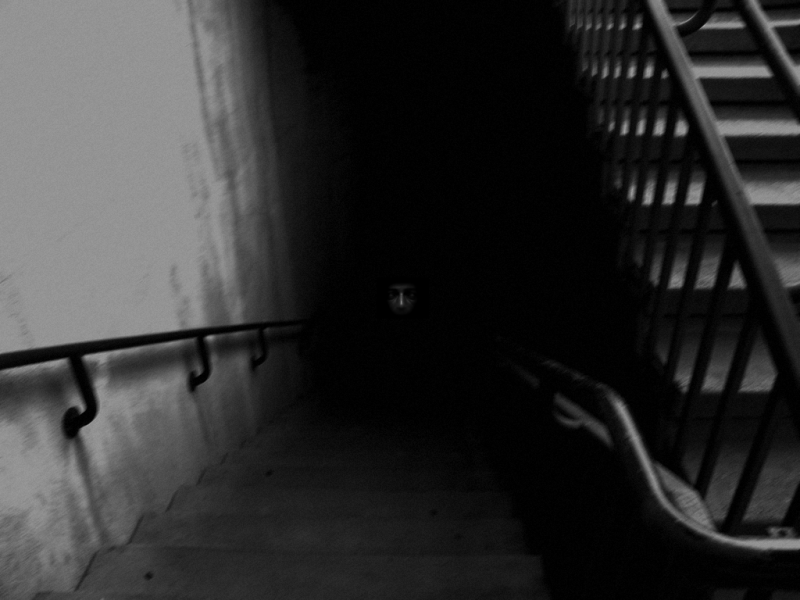
\includegraphics[width=0.5\linewidth]{images/SCP.087.png}
    \caption*{图片A,从第一次探索的录像中截取的静止帧。}
\end{figure}

\bb{项目编号:}SCP-087

\bb{项目等级:}Euclid

\bb{特殊收容措施:}SCP-087位于{[}已编辑]的校园内,通向SCP-087的门廊由带有带电封锁机制的强化钢板构筑而成,此入口已经被伪装成类似于与该建筑设计一致的门卫室。大门的封锁机制不会解除,除非同时施加██伏特的电流并逆时针扭转钥匙。在门的内部,有6厘米厚的工业泡沫填充。

因为最后一次探索的结果(参阅文件087-IV ),现在禁止任何人进入SCP-087。

\bb{描述:} SCP-087是一个无灯的平台楼梯,每层是斜38度的13阶楼梯,楼层之间是一个180度的大概直径3米的半圆平台,由于在SCP-087里面可见度只有1.5个阶梯,并且没有任何的壁灯和窗户,所以任何去探索SCP-087的人员必须配备照明设备,光源75瓦足够,超过75瓦不会有更好的照明效果,因为SCP-087似乎可以吸收过多的光线。

探索人员报告和声音记录证明项目中存在一种令人紧张的声音,类似于介于█岁至██岁孩童的哭声。估测此声音的来源大约位于首个楼梯平台下方200米处。然而,不管怎样继续前进,都不能感觉到在接近这个声音,从第4次探索(也是最后并且下行距离最远的一次)中看,深度是远远超出了现在科学的建筑和地址结构所能达到的深度。至今为止,仍然不能知道SCP-087到底有没有尽头。

\begin{figure}[H]
    \centering
    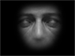
\includegraphics[width=0.5\linewidth]{images/SCP.087.2.png}
    \caption*{图片B,SCP-087-1,放大自第一次探索录像的静止画面。}
\end{figure}

SCP-087至今有4个由D级人员录制的探索录像,每个探险都遭遇到了SCP-087-1(SCP-087里面的未知物体),SCP-087-1是一张没有瞳孔,鼻和嘴的脸,SCP-087-1的性质是完全未知的,但是可以确定他不是哭泣声音的来源,当遇到SCP-087-1的时候,探索人员表现出强烈的疯狂和恐惧,但是很难知道这种反应是反常的还是简单的生理反应。

\bb{附录:}\\
当第4次探险结束后的两周, 有几位来自于{[}已编辑]大学的工作人员和学生都报告称听到SCP-087内部发出频率1-2秒\slash 次的敲击声。SCP-087门口被填充了6厘米的工业泡沫。之后不曾接到对敲击声的报告。

经授权的人员可以参阅文件087-I 到 087-IV,四次探索报告的文件。\\
\hyperref[sec:DOC-document-087-i]{文件087-I}\\
\hyperref[sec:DOC-document-087-ii]{文件087-II}\\
\hyperref[sec:DOC-document-087-iii]{文件087-III}\\
{[}资料被删除]

% SCP 087
\chapter{文件087-I}

\label{chap:DOC-document-087-i}

\bb{文件\#087-I:}探索I

\ii{D-8432是名43岁、外貌平常的白人男性,没什么特殊心理背景,D级称号是因误操作SCP-███而导致降级产生的称号。在探索中,D8432配备了一台75瓦的电量能保持24小时的探照灯,一个手持摄录一体机,并且数据能一直链接到██████博士处,一个与██████博士保持联系的通话耳机。}

\ii{D8432穿过大门走进第一个阶梯,尽管有这么高瓦数的探照灯,灯光仍然只能照到第9个阶梯,下一层是完全看不到的。}

\bb{D-8432:}真他妈的暗!\\
\bb{██████博士:}你的探照灯能起作用吗?

\ii{D-8432 把灯照向门口的学院大厅走廊,这灯光显然可以照到很远的距离。}

\bb{D-8432:}是的,它能起作用,但是不知道怎么回事它就是不能在这些楼梯中照的很远。\\
\bb{██████博士:}谢谢,请继续。

\ii{D-8432走下13步楼梯到达第2个平台,这个平台是半圆的,周围是混泥土墙壁,墙壁上没有什么特殊标记,只是有些尘土和污垢,这显然是很普通的混泥土墙,D-8432转了个弯然后开始向第2层前进,然后停住了。}

\bb{██████博士:}为什么停住?\\
\bb{D-8432:}你听见了吗?这下面他妈有个孩子!

\ii{但是通过设备上的麦克风没有听到D-8432描述的声音。}

\bb{██████博士:}你可以描述一下这个声音吗?\\
\bb{D-8432:}是个很年轻的声音, 可能是女的或者是非常年轻的男孩,她在哭着说\ii{{[}停顿]}请\ii{{[}停顿]}请\ii{{[}停顿]}帮帮我\ii{{[}停顿]}嗯,她就这样哭着一直重复。\\
\bb{██████博士:}你能说下这个声音据你有多远吗?\\
\bb{D-8432:}啊,干,我不知道,大概有200米吧?\\
\bb{██████博士:}请继续走到下一层楼梯。

\ii{对象继续下了13步阶梯,当他到达平台时,孩子的声音从设备里被听见了,这声音夹杂着抽泣,哽咽,一直重复着“请”“救我”“下来”,通过仪器的检测,这声音确实应该是在200米以下。}

\bb{██████博士:}你仍然能听到哭声吗?\\
\bb{D-8432:}是的。\\
\bb{██████博士:}我们已经很好的接收到这个声音了,请继续前进,如果你遇到任何声音或者环境的变化再停住。

\ii{对像在停下前再下了三层楼梯。}

\bb{D-8432:} 我还要继续?\\
\bb{██████博士:}请继续。

\ii{D-8432继续走了17层(目前为止一共下了22层),环境没有任何变化,每层依然是13个阶梯。}

\bb{D-8432:}他妈的,我并没有离那个孩子更近。

\ii{仪器检验这个哭声没有增大,表明依然是在200米以下。}

\bb{██████博士:}我们知道了,但是还是请继续。

\ii{对象继续前进了28层。(目前一共下了50层。) D-8432站在第51层的台阶上,从地面计数来看,D-8432应该已经在门口200米以下了,34分钟过去了,哭声依然没有增大。}

\bb{D-8432:}我感觉很不好。\\
\bb{██████博士:}你在黑暗未知的楼梯中呆了很长时间。这很正常。请继续。

\ii{D-8432很不情愿的继续前进到下一个楼梯,当他继续前进时,在探照灯的的光下,一张脸出现在了下一个楼层底部(SCP-87-1),这张脸与普通人类头部的差不多,但是它没有嘴,鼻孔和瞳孔,这张脸是完全静止的,但是眼睛却直直的盯向D-8432。}

\bb{D-8432:}{[}大叫] 我艹!这他妈是什么东西!干!干你娘!什么鬼!\\
\bb{██████博士:}你能表述下你所看到的吗?\\
\bb{D-8432:}这看起来就像人脸的一部分,它他妈一直在盯着我!它他妈一直在盯着我—\\
\bb{██████博士:}它在动吗?\\
\bb{D-8432:}\ii{{[}停顿,深呼吸]} 没有,它就是盯着我!我艹太可怕了!\\
\bb{██████博士:}请更详细的阐述这个东西。\\
\bb{D-8432:} 不不不,我他妈不想—

\ii{这张脸突然向D-8432移动了大概半米。}

\bb{D-8432:}\ii{{[}尖叫]} 我艹艹艹艹艹艹艹 {[}删除]

\ii{D-8432十分惊恐的开始往回跑,仅仅用了18分钟就跑回了入口,当他崩溃并且往回跑的时候,没有再发现任何关于SCP-87-1的迹象,在返回的过程中,直到跑到快到门口前哭声一直都保持同一个大小,由于惊恐和高速奔跑,D-8432产生了过度疲劳的症状。}

\section{文件087-II}

\label{sec:DOC-document-087-ii}

\bb{文件\#087-II:}探索II

\ii{D-9035是一名强壮的28岁非裔美国男性,除对女性的极度憎恨外无心理异常。目标有大量的{[}数据删除]记录。D-9035 配备了一个可持续亮24小时的100瓦泛光灯, 一个可实时转播的手提摄像机和一个在██████博士控制下用于通信的音频耳机。D-9035还配备了一个装有75个带有胶背、电池寿命可持续约3周的小型LED灯的背包。可通过压缩控制灯泡的明灭。}

\ii{D-9035提着灯照向第一段楼梯,尽管增加了功率,灯光依然只能照亮前9级台阶。}

\bb{D-9035:}博士,你不会让我走下去吧?\\
\bb{██████博士:}请用灯照一下SCP-087外面,确定它功能正常。

\ii{D-9035用灯照向走廊。对比探索I,照明范围确实更大了。}

\bb{██████博士:}谢谢。请往下走到第一个平台。\\
\bb{D-9035:}嘿博士,我知道你的意思,但我不想过去。\\
\bb{██████博士:}请往下走到第一个平台。\\
\bb{D-9035:}博士,是这样,我——\\
\bb{██████博士:}\ii{{[}打断]}像我们之前说的那样,请往下走到第一个平台。

\ii{D-9035停顿了18秒,然后走下13级台阶到了第一个平台停下了。}

\bb{D-9035:}那是个小孩吗?\\
\bb{██████博士:}请拿出一个粘合灯,把它粘在这个平台的墙上。\\
\bb{D-9035:}博士,你听见了吗?下面是不是有个小孩?\\
\bb{██████博士:}我们还未确认这件事,请在墙上粘一个灯泡,然后检查它是否功能正常。

\ii{D-9035犹豫了一会,然后从包里拿出了一个灯泡粘在了墙上。他按了一下灯,灯亮了。}

\bb{██████博士:}请关上你的泛光灯。

\ii{D-9035在关灯前又犹豫了一会。LED灯照亮了平台,但是无论是上行还是下行楼梯的第一级台阶都没有被照亮。}

\bb{██████博士:}谢谢,你可以重新打开你的泛光灯了。请继续往下走。在每个转角的平台上,都要在墙上粘一个LED灯并打开它。如果你注意到了任何不寻常的事,请向我汇报。

\ii{D-9035重新打开了泛光灯,然后走下第二段台阶。当他踏上平台的时候,又响起了恳求和哭泣的声音,与第一次探索一样。}

\bb{██████博士:}你还能听见你刚才报告的那个声音吗?\\
\bb{D-9035:}呃,是的。她听起来在下面大概150,200米处,我是不是要去找到她?博士,我可跟小孩相处不来。\\
\bb{██████博士:}请装好灯,然后继续下行直到你注意到了其他不寻常的事。

\ii{目标在墙上粘好了灯泡并开了灯,然后继续走向下一个平台,粘好并打开了第三个LED灯泡。D-9035又重复了25次同样的动作才停下。}

\bb{D-9035:}博士,我不觉得我靠近了那个孩子。\\
\bb{██████博士:}你估计那个声源还有多远?\\
\bb{D-9035:}和之前一样,在下方150-200米。\\
\bb{██████博士:}谢谢,请继续。

\ii{D-9035又重复之前的行动下了24段楼梯。他在第51个平台处停下了,录像显示混凝土墙上有一个眼形孔洞,约50厘米长,10厘米宽。这个平台下行的第一级台阶似乎完全碎成了瓦砾。}

\bb{D-9035:}你看见那个了吗?\\
\bb{██████博士:}是的,你能描述一下你看见了什么吗?\\
\bb{D-9035:} 看上去像什么东西划坏了这堵墙,然后踩碎了这里的台阶。这个洞看起来很光滑——

\ii{D-9035 摸了摸那个眼形孔洞。}

\bb{D-9035:}哦,它很光滑,像是玻璃。\\
\bb{██████博士:}谢谢,请继续。\\
\bb{D-9035:}博士,我认为我已经走得够远了。\\
\bb{██████博士:}我们有过协议的,请继续走下去。\\
\bb{D-9035:}不管协议怎么说,我都不想做这个了。

{[}数据删除]

\ii{D-9035跨过了被毁的台阶继续往下走。下一个平台没什么特殊的地方,D-9035给接下来的38段楼梯的每个平台都粘了一个LED灯,哭泣和恳求的声音听上去还是一样远。自探索开始,74分钟过去了,D-9035走到了第89个平台处。估计目标处于第一个平台下方350米处。}

\bb{D-9035:}博士,我感觉这孩子只是想引诱我走下去。我认为是时候——

\ii{D-9035不再说话,举起灯照亮了SCP-087-1。那张脸直盯着D-9035,显示它意识到了目标的存在。虽然SCP-087-1看起来没有动,它的位置较探索I中遭遇它的位置下降了38段楼梯,表示它是会移动的。}

\bb{██████博士:}你为什么停下了?\\
\bb{D-9035:}\ii{{[}无回应]}

\ii{D-9035呼吸急促起来。SCP-087-1在接下来的13秒都没有动,然后它眨了眨眼。}

\bb{D-9035:}\ii{{[}大叫,意义不明]}

\ii{SCP-087-1突然冲到了D-9035面前约90厘米处,目标转身逃上楼梯。}

\bb{██████博士:}请冷静下来,转身,我们需要进一步观察那张脸。

\ii{D-9035无视了██████博士并继续跑上楼,持续性发出意义不明的尖叫。}

\bb{██████博士:}D-9035,你能听到我说话吗?请停下来。

\ii{D-9035没有回答,继续跑上楼。他的尖叫声变得嘶哑。在跑上了72段楼梯后,D-9035倒在了第十七层平台上。}

\bb{██████博士:}D-9035,你能听到我吗?

\ii{D-9035无回应,但是通过耳机可以听到他粗重的呼吸声。在接下来的14分钟里,D-9035没有再移动。录像画面一片漆黑,耳机里只有目标的呼吸声和下方不断的恳求声。这种情况持续了14分钟又32秒,然后出现了完全不像人类心跳的快速心跳声和轻微的碎裂声。7秒后,D-9035喘着气苏醒了,无声地继续快速上楼。心跳声和碎裂声停止了,摄像机也没有拍摄到不寻常的画面。在沉默中,D-9035走出了SCP-087,坐在了入口处的地板上。}

\ii{D-9035陷入了神经紧张,尚未恢复。}

\chapter{文件087-III}

\label{chap:DOC-document-087-iii}

\bb{文件\#087-III:}探索III

\ii{D-9884是一位外貌普通、中等体型的23岁女性,有抑郁症病史。目标有不多的通过极端暴力行为 {[}数据删除]的记录。D-9884配备了一个电池可持续24小时的75瓦泛光灯,一个可实时转播的手提摄像机和一个██████博士控制的用于交流的耳机。D-9884还配备了一个装有3.75升水,15条营养棒和一条电热毯的背包。}

\ii{D-9884站在SCP-087最初的平台上,泛光灯只能照亮前9级台阶,上次探索时放下的LED灯已经不见了。}

\bb{██████博士:}请走下第一段楼梯去检查那个平台附近的墙面。

\ii{D-9884往下走了13级台阶,停在了平台上。探索II中放置的LED灯已经消失地无影无踪。}

\bb{D-9884:}好的,嗯,它就是一堵脏兮兮的混凝土墙,上面好像什么都没有。哦不,等一下,这里有点粘粘的。

\ii{D-9884指出了LED灯原本所在的位置。}

\bb{D-9884:}下面有个小孩在哭!她{[}停顿]她在请求帮助。\\
\bb{██████博士:}谢谢,请继续往下走直到你注意到任何不对劲的地方。

\ii{D-9884往下走到第二个平台处,耳机接收到了与前两次探索相同的小孩哭泣声。墙上的LED灯全都不见了,除此之外一切如常,直到D-9884到达了第17个平台。}

\bb{D-9884:}呃,这里地上有一些难闻的东西。它全都黏在我的鞋子上了,呃,真恶心。

\ii{摄像证实了地上有一滩直径约50厘米的物质。}

\bb{██████博士:}你能描述一下那个气味吗?\\
\bb{D-9884:}呃……它闻起来像是生锈的金属和尿液。\\
\bb{██████博士:}谢谢你,请继续走,直到你看到什么别的东西。

\ii{D-9884一路走到了第51个平台,这里看上去和上次探索时一模一样,也观测到了类似的东西。D-9884被要求继续下行直到发现其他的不寻常处。目标继续走到了第89个平台,视频画面猛然一动,目标大叫了起来。}

\bb{D-9884:}啊,草!地上有个洞,我差点掉进去。

\ii{录像显示地上有个直径约一米的洞。目标用泛光灯照下去,只能看到一片黑暗。大约4秒后,洞中不知何处亮了2秒钟又熄灭了。}

\bb{D-9884:}下面有一盏灯!它现在消失了,但是它刚刚好像出现了一秒钟!你看到它了吗?\\
\bb{██████博士:}是的,你觉得这个洞有多深?\\
\bb{D-9884:}不知道,它太深了。至少有一公里,不,远远不止一公里。\\
\bb{██████博士:}谢谢,你还能听到那个小孩的声音吗?\\
\bb{D-9884:}嗯哼,她听上去离我还是很远。我不觉得我更靠近她了,好像我每靠近一步,她就向后退一步。\\
\bb{██████博士:}请接着下楼直到你发现任何不寻常的地方。

\ii{D-9884继续在SCP-087中走了约一小时,又经过了164个平台。她在第253个平台上停下来休息,吃了一根能量棒,喝了几大口水。D-9884处于第一个平台下方约1.1公里处,但是小孩的声音并没有变响。休息了4分钟后,D-9884恢复了下行,不停歇的又走了1.5个小时,216个平台。D-9884现在处于第469个平台上,地下约1.8公里处。}

\bb{D-9884:}我不想再走了,我觉得是时候回去了。我是说,往下走是一回事,但是我回来要爬很久的楼梯呢。\\
\bb{██████博士:}你身上有可以让你在里面待24小时的食物,水和毯子。请继续往下走。\\
\bb{D-9884:} 不,我想我要回来了。

\ii{D-9884转向了刚才下来的楼梯。}

\bb{D-9884:}我——\ii{{[}尖叫]}

\ii{SCP-087-1那张脸就在D-9884背后,阻挡了她回去的道路。那张脸出现在摄像头前方约30厘米处;它的眼神固定在镜头上,这次它没有看着目标,而是看着坐在监控背后的那个人。摄像机的画面故障了4秒,此时耳机里传来持续粗哑的尖叫声。然后摄像机切换到了D-9884急速跑下楼的画面。}

\bb{D-9884:}\ii{{[}慌乱,歇斯底里]}它一直跟着我!这么长的时间里它就在我背后哦天哪它就在我背后这样看着我!██████ 博士求求你做些什么帮帮我哦天哪哦不把它弄走不求求你我知道它一直跟着我求求你把它弄走哦不它在看着我它一直在看着我它知道我在这儿它一直都在看着我哦天哪请帮帮我哦不求求你\ii{{[}这种话一直持续到了最后。]}

\ii{D-9884一边跑下楼梯一边歇斯底里地尖叫、恳求。之前听到的持续粗哑的尖叫声又出现了,在其之下还能听到最初的那个小孩哭泣的声音。大约跑了14段楼梯,摄像头找到了D-9884背后的区域,那张脸现在离镜头只有约20厘米了。它没有看目标;而是注视着镜头,给人一种它正盯着那些观看录像的人看的错觉。值得注意的是,自从SCP-087-1出现后,女孩哭泣恳求的声音变响了,表明D-9884接近了声源。在慌张跑过约150个平台、3次看到SCP-087-1仍在追赶她后,D-9884绊倒了,失去了意识。音频显示此时已经很接近那个哭泣的声源了,而持续粗哑的尖叫声从未间断过。视频显示还有下行的楼梯,D-9884仍未到达底部。画面静止了12秒,然后那张脸占据了整个屏幕,眼睛直勾勾地看着观众。}

\ii{视频和音频中断了,再没能重新连接。}

